% !TEX root = Tesi.tex
\chead{}
\chapter{Background}

\section{Internet of Things and Web}
  
Particularly during the last few years, we have been standing at the forefront of a world where virtually everything can be connected directly to the Internet, an increasingly connected world where emerging technologies enabled objects to be linked among themselves through the usage of new devices and sensors.

This new era of the internet became visible in our everyday lives, from souped-up gadgets tracking our every move to environments capable of predicting our actions and emotions, the list keeps growing every day.


The internet made of things is becoming more central to society than the web as we know it today, this does not necessarily mean the latter is expected to die but rather its role will reduce to that of a language used for displaying content on devices which are supposed to be more ubiquitous but less needed.

The first pioneer species for this ecosystem of "invisible buttons" has certainly been the smartphone. Its increasing usage among the masses made it the perfect candidate for such a revolutionary change. One of the many usages that would help understanding better this pioneering aspect is the way it beams the information about our location and speed when we take it with us in a car, for example, resulting in a real-time traffic information usable by everyone. In such scenario, the actual gathering of real traffic data happens without the user ever being aware of the data transmission and without a real need for interaction such as a click on a button or navigating to a particular web page.

This sort of awareness, especially as it relates to the physical world, leads to areas in space that are listening to the environment and trigger events depending on certain conditions in an entirely automatic way, like a smartphone getting into the range in this case. It could be as small as two centimeters on top of a credit card reader to enable touch payments or as large as rooms which might want to know that we just entered or left so that it can switch on or off the lights.

What is important to notice is that those connected objects are far from being simple on-off switches, they would not be very useful if so. However, because the actions they can potentially trigger can be affected by an endless list of other variables like the time of the day, our personal preferences or actions of others they quickly become a mean to program better and more efficiently our physical world.

Leveraging the usage of a smartphone to act as a proximity sensor is just an artifact of where the technology is nowadays, the same can be accomplished with any number of sensors directly connected to the internet capable of dealing with motion, sound, light temperature, humidity, and others.

Companies like Apple have been embracing the idea of invisible buttons since the beginning of this new era of sensors and devices. 
While the company has been embracing the technology foreseeing its potential from the beginning, it recently rolled out devices called iBeacon. In a nutshell, the beacon allows any newer iPhone or Android phone to know its position in space with centimeter precision. Similarly to a more precise GPS that works indoors, an iBeacon allows the developers to take advantage of the technology to define “invisible buttons” of just about any dimensions.

\vspace{0.5cm}
\begin{figure}[htbp]
  \centering
    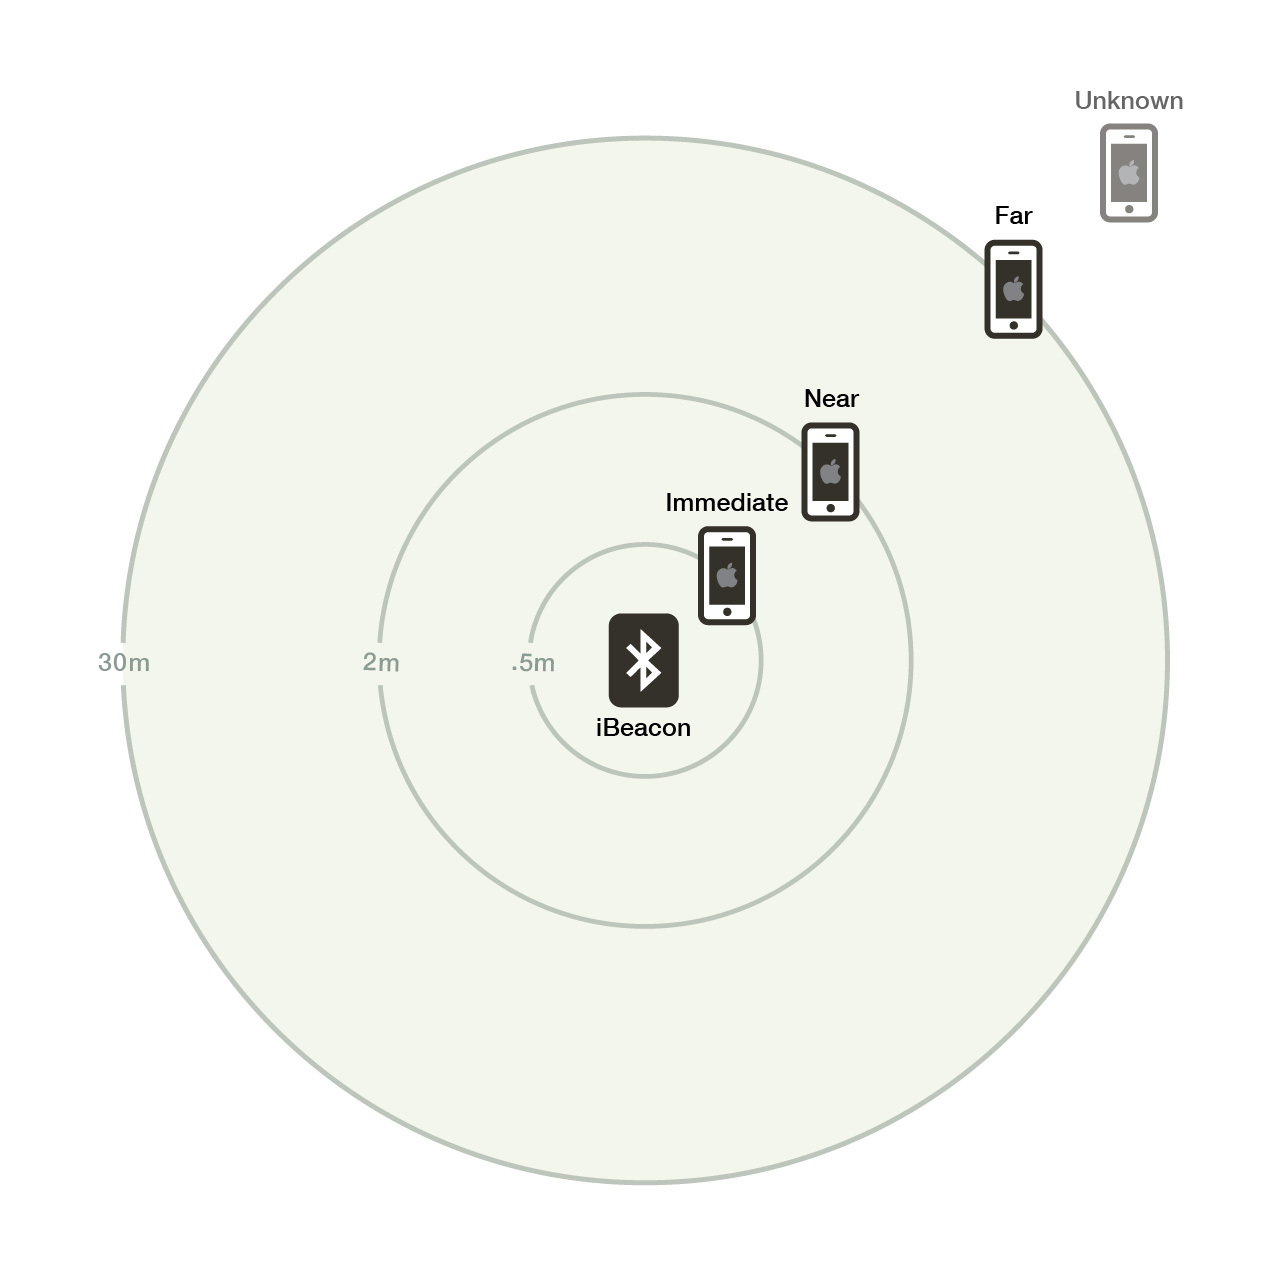
\includegraphics[height=8cm]{images/ibeacon-distance.jpg}
  \caption{Distance categories for iBeacon}
  \label{fig:ibeacon}
\end{figure}
\vspace{0.5cm}


In fact, nothing is stopping this technology from being squeezed into something as small as a typical credit card or being embedded in any clothing or other discrete wearable devices like fitness sensors, wristwatches or even temporary tattoos; the opportunities are indeed countless.

Whether we wear those sensors or use them in our homes and businesses (see smart thermostats, lighting and security systems for example), they can all be prepared and trained to cooperate in sophisticated and unexpected ways once the internet knows that we are present nearby and what our intentions might be. Imagine a smart home capable of knowing when we wake up based on the activity monitor on our wrist and begin warming up the house, brewing a pot of coffee and switching off our security system. 

It is evident that with such a capacity for sensing and responding to our needs,  the internet of things is slowly shaping a brand new world capable of being as alive as it never been before.


\vspace{0.5cm}
\begin{figure}[htbp]
  \centering
    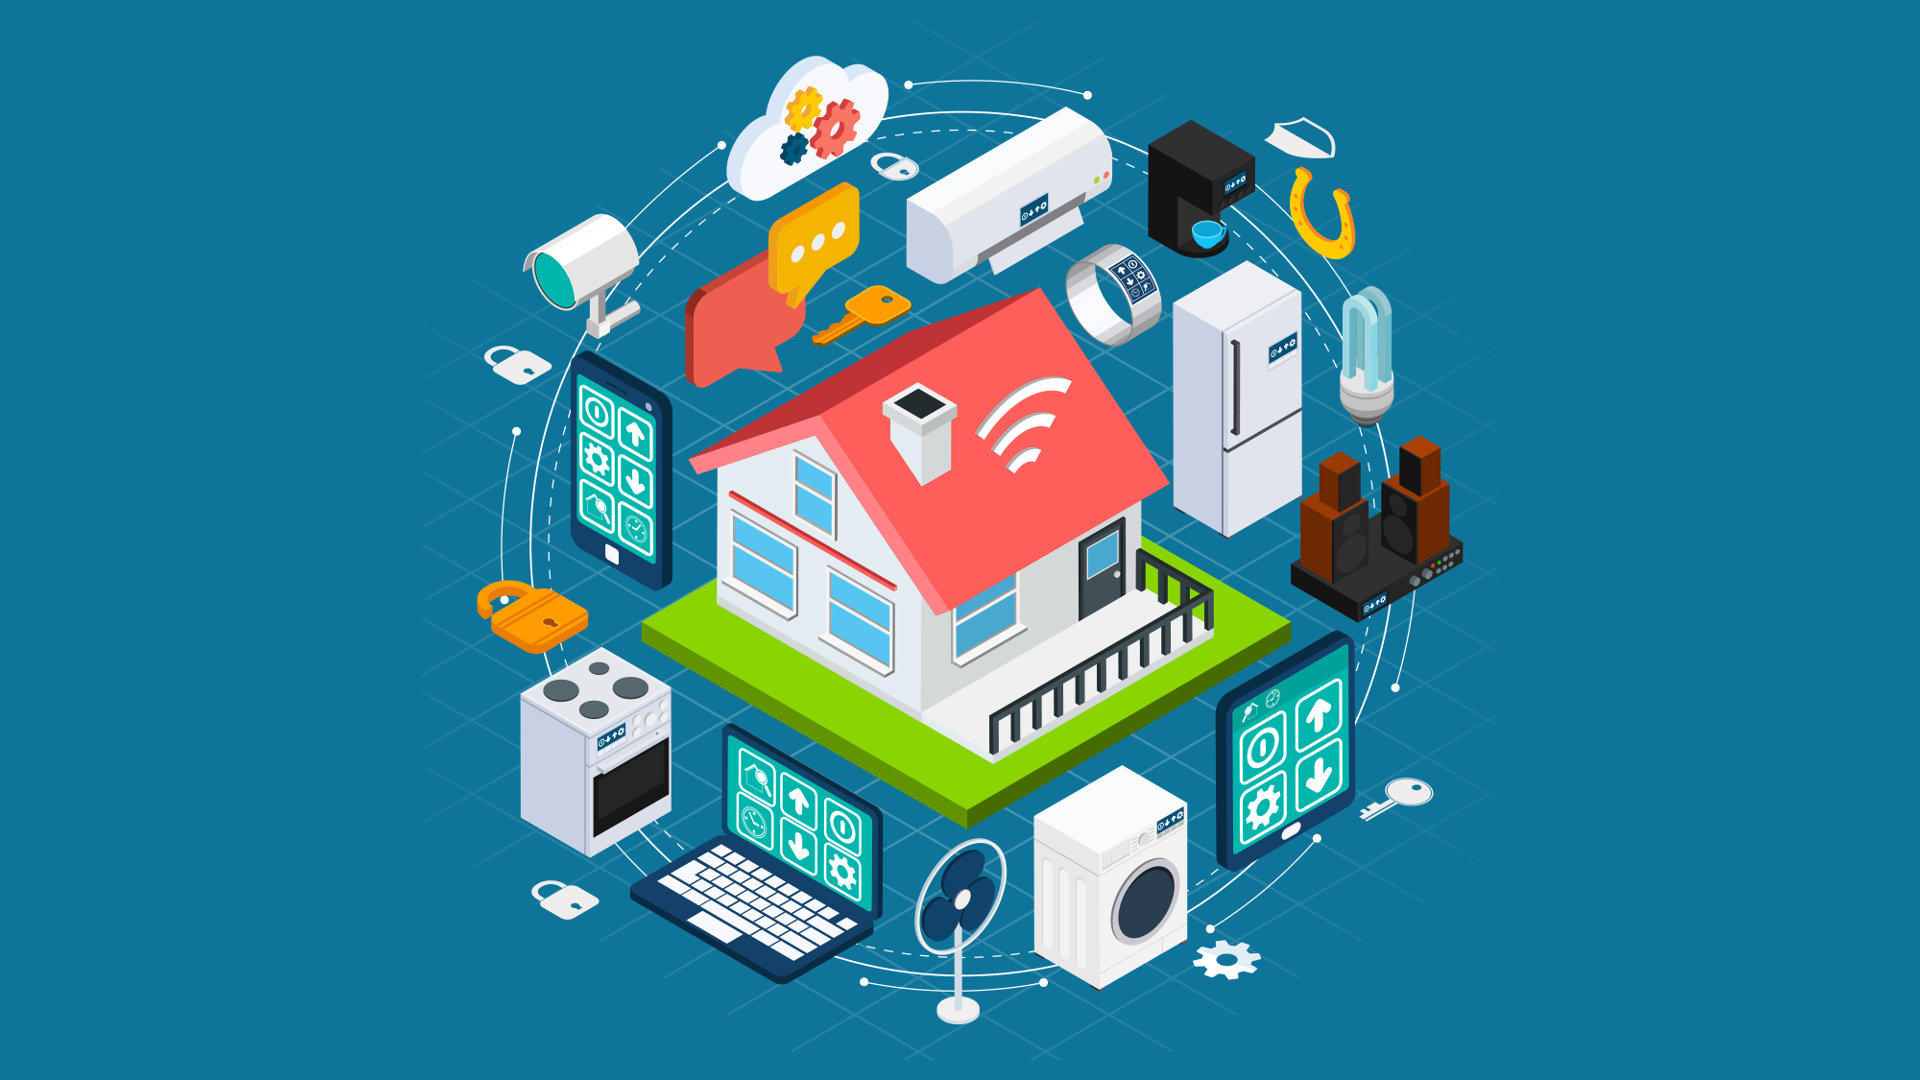
\includegraphics[height=8cm]{images/iot}
  \caption{A smart home ecosystem}
  \label{fig:iot}
\end{figure}
\vspace{0.5cm}

\section{Data and web mining}

Very often company management requires choosing which, among different Business Intelligence solutions available, is the most adequate to fit its need in order to perform crucial strategic decisions.

One of the tools used for this particular goal is certainly a technique called data mining which is the result of a continuous evolution started in the last thirty years of data review.

Up until the late seventies, the Business Intelligence was in charge to play its role through the use of standardized reports which contained simple summarized data and analysis.

In the early eighties, companies started to query in a more detailed and complex way the available data making it easier patterns detection based, for example, on an individual product or geographic area.

Nowadays the advanced software available on the market for the mining is capable of performing patterns detection in real time upon a vast quantity of data thrown at it expediting the company decision making processes and the creation of robust long-term strategies.

\vspace{0.5cm}
\begin{figure}[htbp]
  \centering
    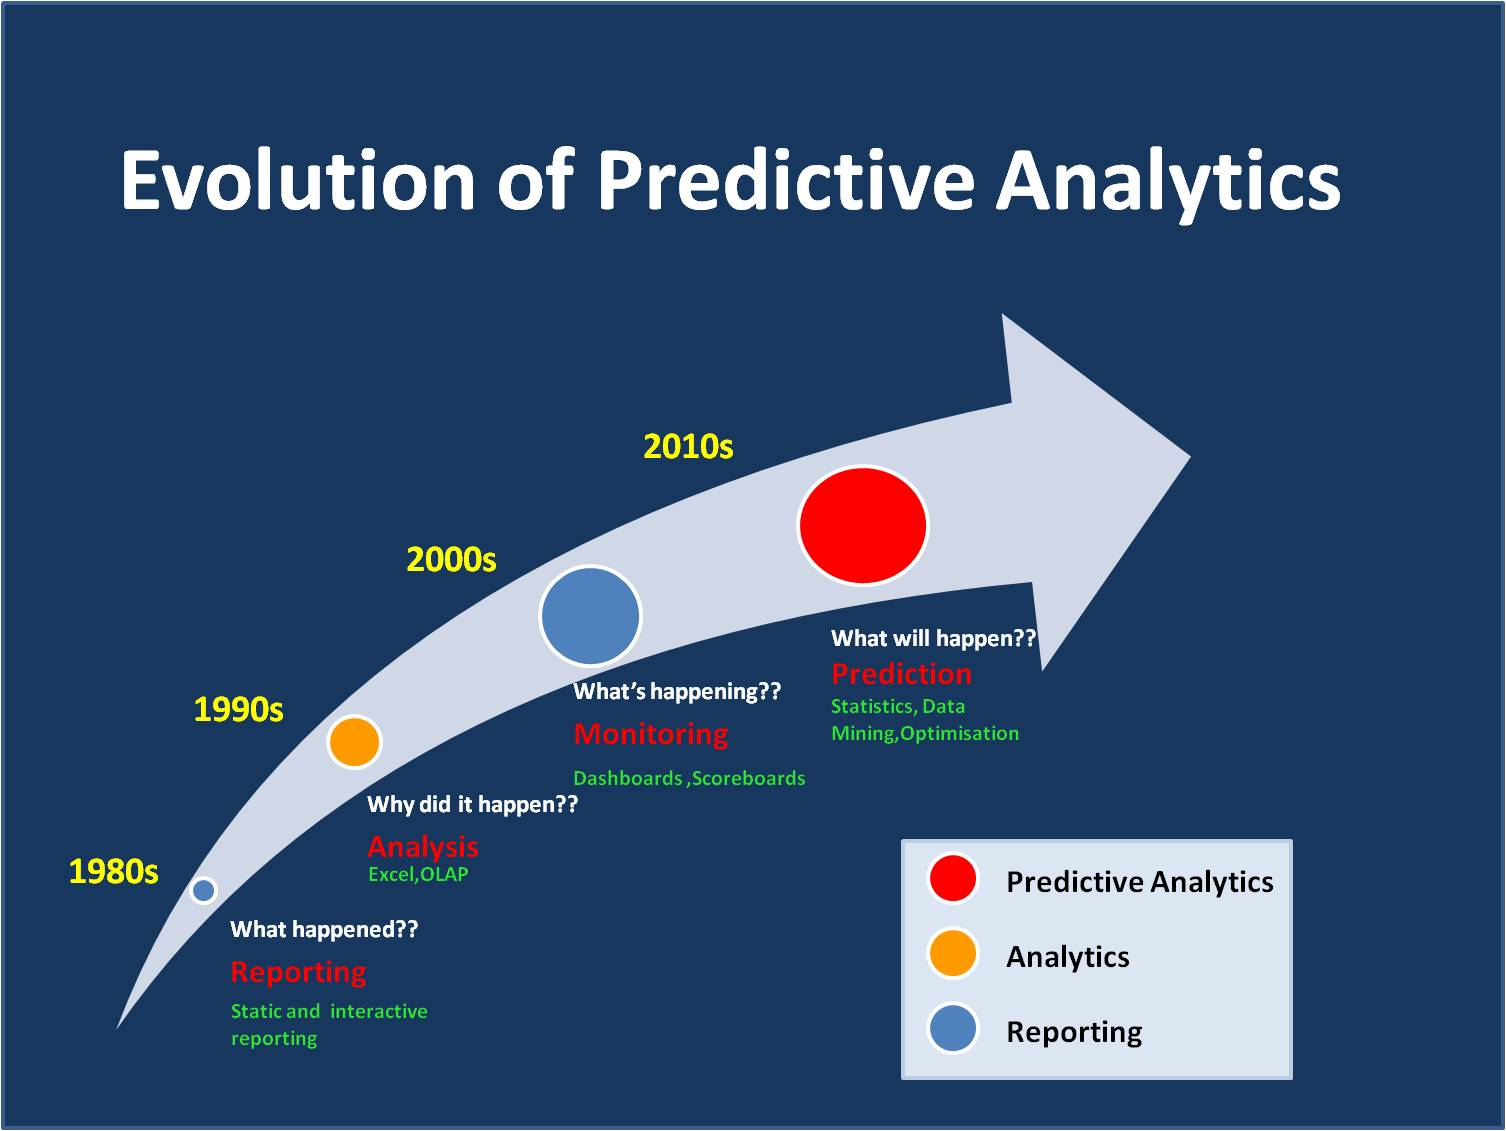
\includegraphics[height=8cm]{images/evolution}
  \caption{Evolution of Predictive Analysis over the last 40 years}
  \label{fig:predict}
\end{figure}
\vspace{0.5cm}
 

Thoroughly interpreting and analyzing the available data, the process of data mining brings better overall understanding and helps taking better decisions.
In fact, thanks to advanced examination techniques, it is possible to find out about hidden information and create analytical models and data groups, identify relationships among activities while correcting errors.

All of this certainly leads to real advantages for a company leveraging this process, both in revenue and cost terms. For example,  on the side of income, the data mining allows to identify and classify the best, real and potential customers, discover additional sales opportunities, increase economic productivity and find new ways and new solutions to grow. In parallel, on the face of the cost, the process could maintain the clientele by identifying customer loyalty elements, reduce exposure to non-payment risks and distribute resources more efficiently.
 
For an organization, the reasons behind the usage of data mining might be different.
The central point is the need to derive insight from the data that will guide the transformation, reorganization or innovation of business processes.
It is evident that decisions based on accurate and reliable knowledge are always the best. Data mining, in fact, provides exactly this type of learning.
While ERP systems improve operational efficiency, they do not provide the strategic drive for business growth or business change. Warehousing systems can efficiently store data, but they lack tools to transform those figures into valuable information focusing on reporting and answering to mostly static questions such as areas where the company sold the most for example. On the other side, data mining tools try to present an interpretation to a wider range of more interesting problems such as the why sales are not taking off as expected, why customers prefer competitors or which previous marketing campaign had the best outcome.

Understanding the answers to these questions means taking the right measures to improve the business performance.
 
Besides data visualization techniques, one of the most popular data mining process on the market is based on the simplified transposition of the neural networks and the neural process of the human brain: when presented with models, it understands that some patterns are associated with other desired results. In the same way, artificial neural networks are capable, by learning about a set of historical data called learning sets, to generate patterns and validate them on another subset of data called test sets.They operate iteratively by modifying patterns from time to time to reach an optimal solution and have the ability to evaluate and provide feedback on unknown data making them very useful for forecasting and classification of knowledge. They very often are presented as a "black box" approach to data mining and they turn out to be very useful when parametric models are difficult to construct and when the emphasis is on foretelling rather than explaining complex patterns.


\vspace{0.5cm}
\begin{figure}[htbp]
  \centering
    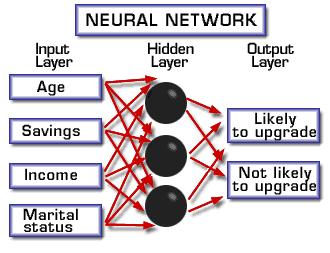
\includegraphics[height=5cm]{images/neural}
  \caption{Neural networks learn to predict outputs after proper training and weighting.}
  \label{fig:neural}
\end{figure}
\vspace{0.5cm}

After discovering what data mining means, which sector uses it the most and how is usually carried over, it is important to focus our attention on the utilization of this tool on the web and its characteristics in such scenario.

In fact, web data mining can detect behavioral models of website visitors, generate reports and implement actions based on those identified patterns.
This process is possible because website visitors often unknowingly provide information about themselves and how they respond to the content presented. Monitoring what links they click, where most of the time is spent, what search terms are looked for and when the visitors leave the website are just an appetizer of the endless stream of possible input data.
Some visitors can also provide information about their lifestyle or names and addresses.
Because of all of this, a thorough and adaptive analysis performed on this considerable amount of stored information is fundamental, and this is exactly where web data mining kicks in helping to design the web shopper behavioral model and making valuable predictions.

One of the features that make up its strength is unquestionably the ability to combine emerging traffic data to the site with those relating to the transactions and the profile of the buyers.
Through these combinations and highlighting the patterns found, it is possible to both gathering complex and strategic considerations and generating predictions that may be indispensable and vital for managing a website that wants to improve its business.

Due to the heterogeneity nature of the source data Web Mining is far from being an application of traditional data mining techniques only, in fact, it can be categorized into three main types:

\begin{itemize}
  \item \textbf{Web structure mining}:  It focuses on analyzing and discovering useful knowledge from hyperlinks representing the structure of the Web. For example from those links, we can detect relevant Web pages as search engines are already doing. Alternatively, it is possible to determine shared common interests among users and so on.
  \item \textbf{Web content mining}: Its main goal is extracting valuable information or data from the content of the web pages. After doing so, it is possible to classify and group them accordingly to their topics automatically. While these tasks are apparently similar to those in traditional data mining, we still can discover relevant behavioral models using products descriptions, forum posts, customer reviews and much more.
  \item \textbf{Web usage mining}: It usually refers to the identification of user access patterns from Web usage logs once the sanitization and preprocessing of the clickstream data has occurred.
\end{itemize} 


\vspace{0.5cm}
\begin{figure}[!htbp]
  \centering
    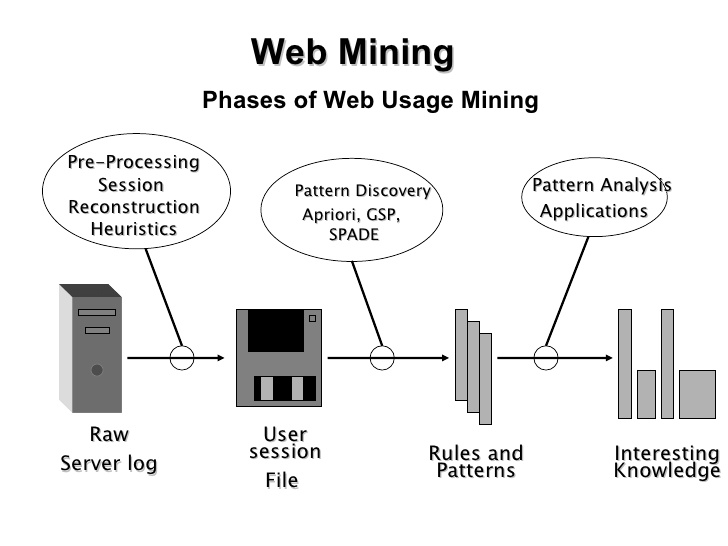
\includegraphics[height=8cm]{images/webmining}
  \caption{Phases of Web Usage Mining}
  \label{fig:webmining}
\end{figure}
\vspace{0.5cm}


Although the web mining process is similar to the traditional data mining one, the data gets collected in an entirely different way. While for traditional data mining the data is often already available stored in a data warehouse, for the web counterpart the effort for the data acquisition can be a cumbersome task, especially for web structure and content mining due to the potentially high number of links and pages to crawl.

\section{Model-driven techniques}



%\addcontentsline{toc}{chapter}{}
